\documentclass[12pt]{article}
\usepackage[margin=1.5cm]{geometry}
\usepackage{parskip}
\usepackage{amsmath}
\usepackage{amssymb}
\usepackage{amsfonts}
\usepackage{enumitem}
\usepackage{graphicx}
\usepackage{stmaryrd}
\graphicspath{ {./images/} }


\begin{document}
\begin{enumerate}[label=(\alph*)]
  \item
    A variable is live at a program point (in the semantic sense), if changing the variable at that program point could affect the I/O behaviour of the program along some possible execution path.

    This is undecidable in general, so we often instead opt for a syntactic version, where we consider all execution paths, regardless of if they are possible or not.

    For example:

\begin{verbatim}
x = input()
if ((x+1) * (x+1) == 0) {
  y = 1
}
if (x*x + 2*x + 1 != 0) {
  y = 2
}
print y
\end{verbatim}

Here, \texttt{y} is not semantically live before the if statements, but is syntactically live. This means that we end up with an overestimation of liveness. This is okay, however, we just have to ensure that the resulting optimisation (such as dead code removal) understands this, and the optimisation will be safe, like it is in dead code removal.

\item
  Unreachable code is code that can never be executed by a program.

  Dead code is code that can still be executed by a program, but whose removal would have no effects on the I/O behaviour of the program.

  To remove unreachable code, we can create a flowgraph of our program, and perform a search from the entrypoint, and then removing code that is not reached by the search.

  To remove dead code, we can use live variable analysis for example to find assignments to non-live variables.

\item
  \begin{enumerate}[label=(\roman*)]
    \item
      Flowgraph is given below:

      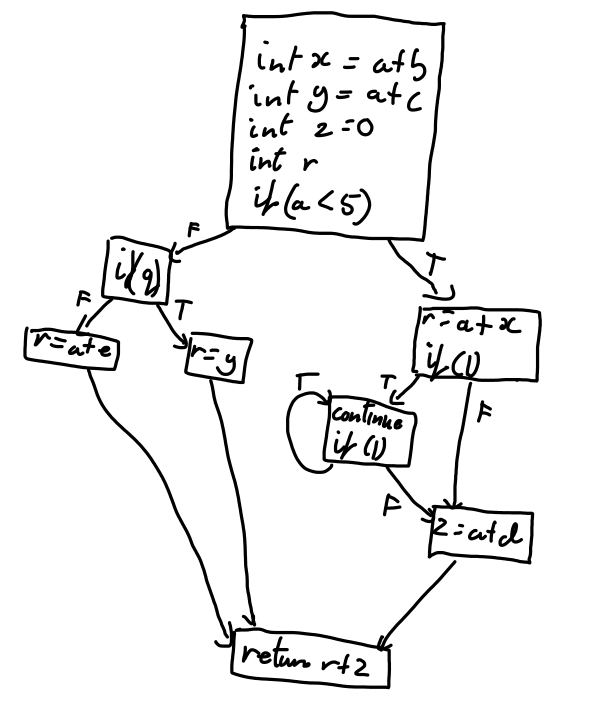
\includegraphics[scale=0.3]{flowgraph}

    \item
      We rewrite the program, providing liveness sets:

\begin{verbatim}
int x = a+b;     {a,b,c,d,e}
int y = a+c;     {a,x,d,e,c}
int z = 0;       {a,x,d,y,e}
int r;           {a,x,d,z,y,e}
if (a < 5) {     {a,x,d,z,y,e}
  r = a + x;     {a,x,d}
  while (1) {
    continue;
  }
  z = a+d;       {r,a,d}
} else if (q) {  {z,y,a,e}
  r = y;         {z,y}
} else {
  r = a + e      {z,a,e}
} 
return r + z     {r,z}

\end{verbatim}

So the set is \texttt{a,b,c,d,e}

For semantic liveness, we notice that the while loop will never terminate, and the final \texttt{else} branch can never be executed, so the semantic liveness set is \texttt{a,c}, which is a subset of the syntactic liveness set.

\item
  We get the following code:

\begin{verbatim}
int y = a+c;
int r;    
if (a < 5) { 
  while (1) {
    continue;
  }
} else if (q) {  
  r = y;        
} else {
  r = a + e    
} 
return r
\end{verbatim}

By analysing the condition of the \texttt{while} loop, we can remove the false branch of the \texttt{if(1)} statements. Then, by applying unreachable code elimination, we remove the \texttt{z = a+d}. Then, dead code elimination lets us remove \texttt{r = a + x} and \texttt{int x = a+b}. Constant propagation then lets  remove \texttt{int z = 0}, and we can then simplify \texttt{r+0} to \texttt{r}.

In this optimised version of \texttt{p}, our syntactic liveness set becomes \texttt{a,c,e} and our semantic liveness set remains \texttt{a,c}.

      
  \end{enumerate}


        
\end{enumerate}
\end{document}
